\documentclass[12pt,a4paper]{article}
\usepackage[utf8]{inputenc}
\usepackage{polski}
\usepackage[polish]{babel}
\usepackage{amsmath}
\usepackage{amsfonts}
\usepackage{amssymb}
\usepackage{graphicx}
\usepackage[export]{adjustbox}
\usepackage{wrapfig}
\usepackage{caption}

\numberwithin{equation}{section}

\renewcommand{\baselinestretch}{1.5}
\captionsetup[figure]{labelformat={default},name={\bfseries Rys.}}
\captionsetup[table]{labelformat={default},name={\bfseries Tab.}}

\newcommand*{\captionsource}[2]{%
	\caption[{#1}]{%
		#1%
		\\\hspace{\linewidth}%
		\textbf{Żródło:} #2%
	}%
}


\title{2. Mostek Wheatstone'a}
\date{25 października 2017}	
\author{
	Zespół 3: Górski Paweł, Sozańska Ada\\
	EAIiIB Informatyka, Rok II
}

\begin{document}
\maketitle
% WPROWADZENIE
\section{Wprowadzenie}
Celem tego doświadczenia jest wyznaczenie nieznanych oporów oraz zweryfikowanie wzorów na opór zastępczy oporników w połączeniach: szeregowym i równoległym, przy wykorzystaniu praw Kirchhoffa oraz prawa Ohma.

\subsection{Prawa Kirchhoffa, prawo Ohma}

Mostek Wheatstone'a jest oparty na trzech fundamentalnych prawach obwodów elektrycznych.

Pierwszym z nich jest \emph{Prądowe Prawo Kirchhoffa}. Dotyczy ono prądów wpływających do węzła obwodu elektrycznego. Mówi ono, że suma algebraiczna prądów wpływających do danego węzła jest równa zeru. Zakładając, że do węzła wpływa $n$ prądów $I_j$, gdzie $j \in \{1,2,~\ldots,~n\}$, prawo to można zapisać następująco:
\begin{equation}
	\sum_{j = 1}^{n} I_j = 0.
	\label{krichoff1}
\end{equation}

\pagebreak
Kolejnym prawem jest \emph{Napięciowe Prawo Kirchhoffa}, które dotyczy spadków napięć w oczku (zamkniętej pętli sieci) obwodu elektrycznego. Mówi ono, że suma spadków napięć na wszystkich elementach w oczku jest równa zeru. Zakładając, że w oczku jest $n$ elementów elektrycznych, prawo to można zapisać następująco:
\begin{equation}
	\sum_{j = 1}^{n} U_j = 0.
	\label{krichoff2}
\end{equation}

Ostatnim prawem jest \emph{Prawo Ohma}, które definiuje zależność natężenia i napięcia prądu. Mówi ono, że stosunek napięcia $U$ między końcami przewodnika do natężenia prądu $I$ w nim płynącego jest wielkością stałą. Wielkość ta jest nazywana opornością. 
\begin{equation}
	R = \frac{U}{I}.
	\label{ohm}
\end{equation}
Prawo to może nie być spełnione w elementach nieliniowych (np. dioda) lub gdy temperatura przewodnika nie jest stała.

\pagebreak
\subsection{Mostek Wheatstone'a}

Mostek Wheatstone'a jest układem do porównywania oporów. Oprócz pomiaru wielkości typowych dla obwodów elektrycznych jest on również wykorzystywany do budowania mierników naprężeń, ciśnień hydrostatycznych czy próżni. 

\begin{figure}[!htb]
	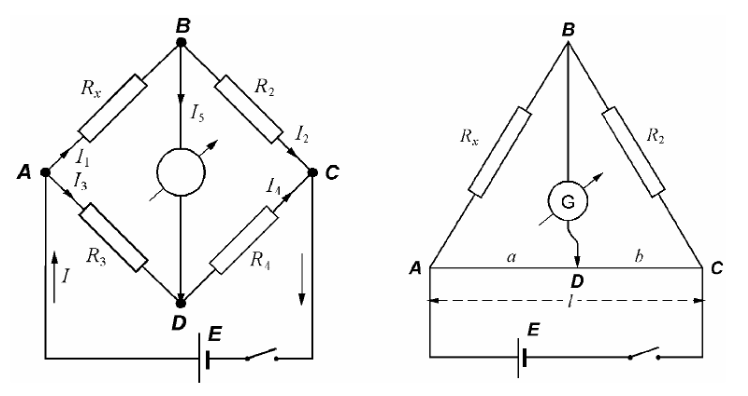
\includegraphics[width=1\textwidth]{img/mostek.png} 
	\captionsource{Schemat mostku Wheatstone'a. Niezrównoważony (po lewej) oraz zrównoważony (po prawej).}{Instrukcja do ćwiczenia}
	\label{fig:img1}
\end{figure}


Składa się on z czterech oporników o porach: $R_x, R_2, R_3, R_4$ oraz galwanometru o oporze $R_5$. Stosując \emph{Prądowe Prawo Kirchhoffa} (\ref{krichoff1}) dla węzłów $B, D$ otrzymujemy następujące równania:
\begin{equation}
	\begin{split}
	&B:~I_1 = I_2 + I_5, \\
	&D:~I_5 = I_3 - I_4.
	\end{split}
	\label{eq:e1}
\end{equation}

\pagebreak
Następnie wykorzystując \emph{Napięciowe Prawo Kirchhoffa} (\ref{krichoff2}) dla oczek $ABDA, BCDB$ otrzymujemy dwa równania:
\begin{equation}
	\begin{split}
	ABDA:&~I_1 R_x + I_5 R_5 - I_3 R_3 = 0, \\
	BCDB:&~I_2 R_2 - I_4 R_4 - I_5 R_5 = 0.
	\end{split}
	\label{eq:e2}
\end{equation}

W doświadczeniu wykorzystujemy układ zrównoważony, w którym potencjały w węzłach $B$ i $D$ są równe. W konsekwencji mamy $I_5 = 0$, co powoduje uproszczenie układu równań (\ref{eq:e1}) do:
\begin{equation}
	\begin{split}
	I_1 = I_2, \\
	I_3 = I_4.
	\end{split}
\end{equation}
Dalej, równania (\ref{eq:e2}) upraszczają się do postaci:
\begin{equation}
	\begin{split}
	I_1 R_x = I_3 R_3 , \\
	I_1 R_2 = I_3 R_4.
	\end{split}
\end{equation}
Co nam daje:
\begin{equation}
	R_x = R_2\frac{R_3}{R_4}
	\label{eq:e3}
\end{equation}

W mostku zrównoważonym opory $R_3$ oraz $R_4$ są oporami wewnętrznymi przewodów o długości kolejno $a$ oraz $b = l - a$ (Rys. \ref{fig:img1}). Opory te można przedstawić wzorami:
\begin{equation}
		R_3 = \rho\frac{a}{S}~~\textrm{oraz}~~R_4 = \rho \frac{l - a}{S},
		\label{eq:e4}
\end{equation}
gdzie $\rho$ to oporność właściwa, a $S$ to pole przekroju wewnętrznego przewodu.

Ostatecznie, korzystając z (\ref{eq:e3}) i (\ref{eq:e4}) otrzymujemy wzór, w którym wszystkie parametry są mierzalne:
\begin{equation}
	R_x = R_2 \frac{a}{l - a}
\end{equation}

\pagebreak
% WYKONANIE ĆWICZENIA
\section{Wykonanie ćwiczenia}


W celu wykonania doświadczenia wykorzystaliśmy:
\begin{itemize}
	\item Listwę o długości $1$~m z podziałką milimetrową, drutem oporowym i suwakiem,
	\item Opornicę dekadową $R$,
	\item Zestaw oporników $R_x$,
	\item Mikroamperomierz,
	\item Zasilacz stabilizowany $3$~A/$30$~V.
\end{itemize}

Doświadczenie rozpoczęliśmy od połączenia elementów w zrównoważony mostek Wheatstone'a. Suwak na listwie przesunęliśmy do połowy jej długości ($a = 50$~cm). Dla każdego z oporników $R_x$ ustawialiśmy opór $R$ na opornicy dekadowej tak, aby amperomierz wskazywał $0$~A. Następnie osiem razy zmienialiśmy opór $R$, żeby oscylował w okół wartości początkowej $R$ (ustawionej dla $a = 50$~cm) i dostosowywaliśmy suwak, tak aby za każdym razem amperomierz wskazywał $0$ A.

Analogiczne pomiary wykonaliśmy dla połączenia szeregowego \mbox{($R_{x1}$ z $R_{x2}$)}, równoległego ($R_{x1}$ z $R_{x2}$) i mieszanego ($R_{x3}$ szeregowo z równolegle połączonymi $R_{x1}$ z $R_{x2}$)

\pagebreak
% OPRACOWANIE DANYCH POMIAROWYCH
\section{Opracowanie danych pomiarowych}
\subsection{Pomiary}
Zmierzona długość wahadła wynosi $l = 341$ mm. Niepewność pomiaru długości wahadła $l$ wynosi $u(l) = 1$ mm, ponieważ jest to najmniejsza działka elementarna wykorzystanego narzędzia.

\begin{table}[!ht]
	\caption{Wartości pomiarów okresów wahadła dla stałej długości}
	\begin{center}
		\begin{tabular}{r|r|r|r}
			\hline
			\multicolumn{1}{c|}{L.p.} & \multicolumn{1}{c|}{liczba okresów $k$} & \multicolumn{1}{c|}{czas $t$ dla $k$ okresów [s]} & \multicolumn{1}{c}{okres $T_i = t/k$ [s]} \\ \hline \hline
			1 & 20 & 22,61 & 1,130 \\
			2 & 20 & 22,88 & 1,144 \\
			3 & 20 & 22,64 & 1,132 \\
			4 & 20 & 22,78 & 1,139 \\
			5 & 20 & 22,77 & 1,138 \\
			6 & 20 & 22,88 & 1,144 \\
			7 & 20 & 23,09 & 1,154 \\
			8 & 20 & 23,07 & 1,153 \\
			9 & 20 & 23,15 & 1,157 \\
			10 & 20 & 23,24 & 1,162 \\ \hline
		\end{tabular}
	\end{center}
	\label{tab:tab1}
\end{table}
Wartość średnia okresu $T$ dla wyników pomiaru okresu $T_i$ (Tab. \ref{tab:tab1}) jest równa $T = 1,145~\textrm{s}$. 

Korzystając ze wzoru (\ref{eq:std_uncert}) niepewność pomiaru $u(T)$ jest równa
\begin{equation}
	u(T) = \sqrt{\frac{\sum_{i=1}^{10}(T_i - T)^2}{n(n-1)}},
\end{equation}

Dla danych z tabli otrzymujemy wynik $u(T) = 0,0034$ s.

Poniżej znajdują się wyniki pomiarów (Tab. \ref{tab:tab2}) przy zmiennej długości wahadła potrzebne do wykonania regresji liniowej.
\begin{table}[!ht]
	\caption{Wartości pomiarów okresów wahadła dla zmiennej długości}
	\begin{center}
		\begin{tabular}{r|r|r|r|r|r}
			\hline
			\multicolumn{1}{c|}{L.p.} & \multicolumn{1}{c|}{$l$ [mm]} & \multicolumn{1}{c|}{k} & \multicolumn{1}{c|}{$t$ [s]} & \multicolumn{1}{c|}{$T_i$ [s]} & \multicolumn{1}{c}{$T_{i}^{2} ~[\textrm{s}^2]$} \\ \hline \hline
			1 & 439 & 20 & 26,2 & 1,310 & 1,716 \\
			2 & 403 & 20 & 24,9 & 1,245 & 1,550 \\
			3 & 366 & 20 & 23,68 & 1,184 & 1,401 \\
			4 & 327 & 20 & 22,55 & 1,127 & 1,270 \\
			5 & 285 & 20 & 21,16 & 1,058 & 1,119\\
			6 & 241 & 20 & 19,32 & 0,9660 & 0,9331 \\
			7 & 194 & 20 & 17,87 & 0,8935 & 0,7983 \\
			8 & 153 & 20 & 15,19 & 0,7595 & 0,5768 \\
			9 & 108 & 20 & 13,21 & 0,6605 & 0,4362 \\
			10 & 63 & 20 & 10,34 & 0,5170 & 0,2672 \\ \hline
		\end{tabular}
	\end{center}
	\label{tab:tab2}
\end{table}

\pagebreak
\subsection{Analiza wyniku dla stałej długości wahadła}
Wartość przyspieszenia ziemskiego $g$ dla długości wahadła $l$ oraz okresu wahadła $T$ wynosi:
\begin{equation}
	\begin{split}
		&l = 0,341~\textrm{m},~~T = 1,145~\textrm{s}, \\ 
		&g = 4\pi^2\frac{l}{T^2} \approx 10,26~\frac{\textrm{m}}{\textrm{s}^2}.
	\end{split}
\end{equation}

Korzystając ze wzoru (\ref{eq:uc}) na niepewność złożoną otrzymujemy:
\begin{equation}
	\begin{split}
	u_c(g) & = \sqrt{\Bigg(\frac{4\pi^2}{T^2}u(l)\Bigg)^2 + \Bigg(-8\pi^2\frac{l}{T^3}u(T)\Bigg)^2} \\
	 	   & \approx \sqrt{9,06 \cdot 10^{-4} + 37,82 \cdot 10^{-4}} \\ & \approx0,068~\Big[\frac{\textrm{m}}{\textrm{s}^2}\Big]
	\end{split}
\end{equation}

Niepewność złożona $u_c(g)$ oraz niepewność rozszerzona $U(g)$ (wzór \ref{eq:uc_exp}) wynoszą:
\begin{align}
	u_c(g) = 0,068~\frac{\textrm{m}}{\textrm{s}^2},\\
	U(g) = 0,136~\frac{\textrm{m}}{\textrm{s}^2}.
\end{align}

Wartość tabelaryczna przyspieszenia ziemskiego w Krakowie wynosi $g_0 = 9,811~\frac{\textrm{m}}{\textrm{s}^2}$.

\begin{equation}
	|g - g_0| = 0,37 > U(g) = 0,136~\Big[\frac{\textrm{m}}{\textrm{s}^2}\Big]
	\label{eq:gconst}
\end{equation}

Wynik wskazuje na to, że mógł zostać popełniony błąd systematyczny podczas pomiarów okresów wahadła (żadne dane nie odbiegają od siebie w znaczący sposób). Prawdopodobnie wynika on z braku synchronizacji osób przeprowadzających doświadczenie.

\pagebreak
\subsection{Analiza wyniku dla zmiennej długości wahadła}


Wykorzystując metodę najmniejszych kwadratów przypasowaliśmy następującą prostą:
\begin{equation}
	\begin{split}
	&y = ax,~~ a = 3,888~\Big[\frac{\textrm{s}^2}{\textrm{m}}\Big],\\ 
	&u(a) = 0,023~\Big[\frac{\textrm{s}^2}{\textrm{m}}\Big].
	\end{split}
\end{equation}

\pagebreak
Korzystając ze wzoru:
\begin{equation}
	g = \frac{4\pi^2}{a}
\end{equation}
wyliczamy wartość przyspieszenia ziemskiego $g = 10,15~\frac{\textrm{m}}{\textrm{s}^2}$.


Korzystając z równania (\ref{eq:uc_single}) mamy:
\begin{equation}
	\begin{split}
	u_c(g) = \Big|-\frac{4\pi^2}{a^2}u(a)\Big| & \approx 2,61 \cdot 0,023\\
		   & \approx 0,060~\Big[\frac{\textrm{m}}{\textrm{s}^2}\Big]
	\end{split}
\end{equation}

Niepewność złożona $u_c(g)$ oraz niepewność rozszerzona $U(g)$ pomiaru wynoszą:
\begin{align}
	u_c(g) = 0,060~\frac{\textrm{m}}{\textrm{s}^2}, \\
	U(g) = 0,120~\frac{\textrm{m}}{\textrm{s}^2}.
\end{align}

Porównując z wartością tabelaryczną jak poprzednio mamy:
\begin{equation}
	|g - g_0| = 0,26 > U(g) = 0,120~\Big[\frac{\textrm{m}}{\textrm{s}^2}\Big].
	\label{eq:gvar}
\end{equation}
Ponownie otrzymana wartość przyspieszenia ziemskiego $g$ nie jest zgodna z wartością tabelaryczną.
\section{Wnioski}
Mimo zmniejszenia czynnika ludzkiego (10 pomiarów 20 okresów) oraz wyliczenia średniej ze zmierzonych wartości w celu zminimalizowania niepewności, wyniki otrzymane przy pomocy obu metod nie są zgodne z wartością tabelaryczną dla Krakowa.

Dla naszych danych, metoda druga (wykorzystująca regresję liniową) cechuje się większą dokładnością (\ref{eq:gvar}) aniżeli metoda pierwsza (\ref{eq:gconst}).

Zmierzone wartości okresów musiały być obarczone błędem systematycznym. Błąd ten mógł być spowodowany brakiem synchronizacji eksperymentatorów lub zbyt dużym kątem odchylenia wahadła (większym niż $3^\circ$), bowiem wtedy aproksymacja, którą wykorzystujemy ma większy błąd (zwiększenie kąta z $3^\circ$ do $15^\circ$ powoduje ok. dwudziestokrotnie większy błąd).

%metoda druga (wykorzystująca regresję liniową) cechuje się większą dokładnością (równanie \ref{eq:gvar}) aniżeli metoda pierwsza (równanie \ref{eq:gconst}), której niepewność otrzymanego wyniku jest ponad trzykrotnie większa od niepewności metody drugiej.

%Różnice powstałe między tymi dwoma metodami są spowodowane błędem systematycznym nie wykrytym podczas pomiarów okresu wahadła lub nieprawidłowym przeprowadzeniem doświadczenia. Drastyczny wpływ na wynik mógł mieć zbyt duży kąt odchylenia wahadła (większy niż $3^\circ$), bowiem wtedy aproksymacja, którą wykorzystujemy ma większy błąd (zwiększenie z $3^\circ$ do $15^\circ$ powoduje ok. dwudziestokrotnie większy błąd).
\end{document}